\documentclass{article}
\usepackage{a4wide,stex-logo}
\usepackage{textcomp,url,array,float,amsfonts}
\usepackage{listings}
\usepackage{tikz}
\usepackage[show]{ed}
\usepackage[backref=true,hyperref=auto,style=alphabetic,backend=bibtex]{biblatex}
\bibliography{kwarc}
\usepackage{hyperref}
\makeindex
\floatstyle{boxed}
\newfloat{exfig}{thp}{lop}
\floatname{exfig}{Example}

\def\ctancitesuffix{:ctan}
\def\ctancite#1{\cite{#1\ctancitesuffix}}
\def\meta#1{\textlangle\textit{#1}\textrangle}
\def\scsys#1{{{\sc #1}}\index{#1@{\sc #1}}}
\def\xslt{{\scsys{xslt}}}
\def\xml{\scsys{Xml}}
\def\mathml{\scsys{MathML}}
\def\omdoc{\scsys{OMDoc}}
\def\physml{\scsys{PhysML}}
\def\openmath{\scsys{OpenMath}}
\def\connexions{\scsys{Connexions}}
\def\latexml{\scsys{LaTeXML}}
\def\perl{\scsys{Perl}}
\def\cmathml{Content-{\sc MathML}\index{Content {\sc MathML}}\index{MathML@{\sc MathML}!content}}
\def\activemath{\scsys{ActiveMath}}
\def\twin#1#2{\index{#1!#2}\index{#2!#1}}
\def\twintoo#1#2{{#1 #2}\twin{#1}{#2}}
\def\atwin#1#2#3{\index{#1!#2!#3}\index{#3!#2 (#1)}}
\def\atwintoo#1#2#3{{#1 #2 #3}\atwin{#1}{#2}{#3}}

% these macros are used in the short descriptions
\def\connexions{\scshape{Connexions}}
\def\cnxlatex{CNX\LaTeX}
\def\cnxml{\scshape{CNXml}}

\title{{\stex}: Semantic Markup  in {\TeX/\LaTeX}}
\author{Michael Kohlhase\\
  Jacobs University, Bremen\\
  \url{http://kwarc.info/kohlhase}}
\lstset{columns=fullflexible}
\lstdefinelanguage{MathML}[]{XML}%
{morekeywords={math,semantics,annotation-xml,annotation,
               maction,
               mrow,mo,mi,mn,
               bind,apply,bvar,ci,cn,sep,csymbol,
               condition,domainofapplication,lowlimit,uplimit,degree,
               interval,inverse,lambda,compose,ident,domain,codomain,image,
               piecewise, piece, otherwise,
               quotient,factorial,divide,max,min,minus,plus,power,rem,times, root,gcd,lcm,
               and,or,xor,not,implies,forall,exists,
               abs,conjugate,arg,real,imaginary,floor,ceiling,
               sin,cos,tan,sec,csc,cot,sinh,cosh,tanh,sech,csch,coth,
               arcsin,arccos,arctan,arccosh,arccot,arccoth,arccsc,arccsch,arcsec,arcsech,arcsinh,arctanh,
               eq,neq,gt,lt,geq,leq,equivalent,approx,factorof,
               int,diff,partialdiff,divergence,grad,curl,laplacian,
               set,list,union,intersect,in,notin,subset,prsubset,notsubset,notprsubset,setdiff,card,cartesianproduct,
               sum,product,limit,tendsto,exp,ln,log,mean,sdev,variance,median,mode,moment,momentabout,
               vector,matrix,matrixrow,determinant,transpose,selector,vectorproduct,scalarproduct,outerproduct,
               integers,reals,rationals,naturalnumbers,complexes,primes,
               exponentiale,imaginaryi,notanumber,true,false,emptyset,pi,eulergamma,infinity,
              reln,fn,declare},
   sensitive=true}

\begin{document}
 \pagenumbering{roman}
 \maketitle
\begin{abstract}
  We present a collection of {\TeX} macro packages that allow to markup {\TeX/\LaTeX}
  documents semantically without leaving the document format, essentially turning
  {\TeX/\LaTeX} into a document format for mathematical knowledge management (MKM).
 \end{abstract}
\setcounter{tocdepth}{2}\tableofcontents
\clearpage
\pagenumbering{arabic}

\section{Introduction}

The last few years have seen the emergence of various content-oriented {\xml}-based,
content-oriented markup languages for mathematics on the web, e.g.
{\openmath}~\cite{BusCapCar:2oms04}, {\cmathml}~\cite{CarIon:MathML03}, or our own
{\omdoc}~\cite{Kohlhase:OMDoc1.2}. These representation languages for mathematics, that
make the structure of the mathematical knowledge in a document explicit enough that
machines can operate on it. Other examples of content-oriented formats for mathematics
include the various logic-based languages found in automated reasoning tools
(see~\cite{RobVor:hoar01} for an overview), program specification languages (see
e.g.~\cite{Bergstra:as89}).

The promise if these content-oriented approaches is that various tasks involved in ``doing
mathematics'' (e.g. search, navigation, cross-referencing, quality control, user-adaptive
presentation, proving, simulation) can be machine-supported, and thus the working
mathematician is relieved to do what humans can still do infinitely better than machines:
The creative part of mathematics --- inventing interesting mathematical objects,
conjecturing about their properties and coming up with creative ideas for proving these
conjectures. However, before these promises can be delivered upon (there is even a
conference series~\cite{MKM-IG-Meetings:online} studying ``Mathematical Knowledge
Management (MKM)''), large bodies of mathematical knowledge have to be converted into
content form.

Even though {\mathml} is viewed by most as the coming standard for representing
mathematics on the web and in scientific publications, it has not not fully taken off in
practice. One of the reasons for that may be that the technical communities that need
high-quality methods for publishing mathematics already have an established method which
yields excellent results: the {\TeX/\LaTeX} system: and a large part of mathematical
knowledge is prepared in the form of {\TeX}/{\LaTeX} documents.

{\TeX}~\cite{Knuth:ttb84} is a document presentation format that combines complex
page-description primitives with a powerful macro-expansion facility, which is utilized in
{\LaTeX} (essentially a set of {\TeX} macro packages, see~\cite{Lamport:ladps94}) to
achieve more content-oriented markup that can be adapted to particular tastes via
specialized document styles. It is safe to say that {\LaTeX} largely restricts content
markup to the document structure\footnote{supplying macros e.g. for sections, paragraphs,
  theorems, definitions, etc.}, and graphics, leaving the user with the presentational
{\TeX} primitives for mathematical formulae. Therefore, even though {\LaTeX} goes a great
step into the direction of an MKM format, it is not, as it lacks infrastructure for
marking up the functional structure of formulae and mathematical statements, and their
dependence on and contribution to the mathematical context.

\subsection{The {\xml} vs. {\TeX/\LaTeX} Formats and Workflows}

{\mathml} is an {\xml}-based markup format for mathematical formulae, it is standardized
by the World Wide Web Consortium in {\cite{CarIon:MathML03}}, and is supported by the
major browsers. The {\mathml} format comes in two integrated components: presentation
{\mathml}\twin{presentation}{MathML} and content {\mathml}\twin{content}{MathML}. The
former provides a comprehensive set of layout primitives for presenting the visual
appearance of mathematical formulae, and the second one the functional/logical structure
of the conveyed mathematical objects. For all practical concerns, presentation {\mathml}
is equivalent to the math mode of {\TeX}. The text mode facilitates of {\TeX} (and the
multitude of {\LaTeX} classes) are relegated to other {\xml} formats, which embed
{\mathml}.
 
The programming language constructs of {\TeX} (i.e. the macro definition
facilities\footnote{We count the parser manipulation facilities of {\TeX}, e.g. category
  code changes into the programming facilities as well, these are of course impossible for
  {\mathml}, since it is bound to {\xml} syntax.}) are relegated to the {\xml}
programming languages that can be used to develop language extensions. 
transformation language {\xslt}~\cite{Deach:exls99,Kay:xpr00} or proper {\xml}-enabled
The {\xml}-based syntax and the separation of the presentational-, functional- and
programming/extensibility concerns in {\mathml} has some distinct advantages over the
integrated approach in {\TeX/\LaTeX} on the services side: {\mathml} gives us better
\begin{itemize}
\item integration with web-based publishing,
\item accessibility to disabled persons, e.g. (well-written) {\mathml} contains enough
  structural information to supports screen readers.
\item reusability, searchabiliby and integration with mathematical software systems
  (e.g. copy-and-paste to computer algebra systems), and
\item validation and plausibility checking.
\end{itemize}
 
On the other hand, {\TeX/\LaTeX}/s adaptable syntax and tightly integrated programming
features within has distinct advantages on the authoring side:
  
\begin{itemize}
\item The {\TeX/\LaTeX} syntax is much more compact than {\mathml} (see the difference in
  Figure~\ref{fig:mathml-sum} and Equation ~\ref{eq:cmathml-sum}), and if needed, the
  community develops {\LaTeX} packages that supply new functionality in with a succinct
  and intuitive syntax.
\item The user can define ad-hoc abbreviations and bind them to new control sequences to
  structure the source code.
\item The {\TeX/\LaTeX} community has a vast collection of language extensions and best
  practice examples for every conceivable publication purpose and an established and very
  active developer community that supports these.
\item There is a host of software systems centered around the {\TeX/\LaTeX} language that
  make authoring content easier: many editors have special modes for {\LaTeX}, there are
  spelling/style/grammar checkers, transformers to other markup formats, etc.
\end{itemize}
 
In other words, the technical community is is heavily invested in the whole
{\index*{workflow}}, and technical know-how about the format permeates the
community. Since all of this would need to be re-established for a {\mathml}-based
workflow, the technical community is slow to take up {\mathml} over {\TeX/\LaTeX}, even in
light of the advantages detailed above.
 
\subsection{A {\LaTeX}-based Workflow for {\xml}-based Mathematical Documents}
 
An elegant way of sidestepping most of the problems inherent in transitioning from a
{\LaTeX}-based to an {\xml}-based workflow is to combine both and take advantage of the
respective advantages.
 
The key ingredient in this approach is a system that can transform {\TeX\LaTeX} documents
to their corresponding {\xml}-based counterparts. That way, {\xml}-documents can be
authored and prototyped in the {\LaTeX} workflow, and transformed to {\xml} for
publication and added-value services, combining the two workflows. 
 
There are various attempts to solve the {\TeX/\LaTeX} to {\xml} transformation problem
(see ~\cite{StaGinDav:maacl09} for an overview); the most mature is probably Bruce
Miller's {\latexml} system~\cite{Miller:latexml:online}. It consists of two parts: a
re-implementation of the {\TeX} {\index*{analyzer}} with all of it's intricacies, and a
extensible {\xml} emitter (the component that assembles the output of the parser). Since
the {\LaTeX} style files are (ultimately) programmed in {\TeX}, the {\TeX} analyzer can
handle all {\TeX} extensions, including all of {\LaTeX}. Thus the {\latexml} parser can
handle all of {\TeX/\LaTeX}, if the emitter is extensible, which is guaranteed by the
{\latexml} binding language: To transform a {\TeX/\LaTeX} document to a given {\xml}
format, all {\TeX} extensions\footnote{i.e. all macros, environments, and syntax
  extensions used int the source document} must have ``{\latexml}
bindings''\index{LaTeXML}{binding}, i.e. a directive to the {\latexml} emitter that
specifies the target representation in {\xml}.

\section{The Packages of the \protect\stex Collection}\label{sec:packages}

In the following, we will shortly preview the packages and classes in the {\stex}
collection. They all provide part of the solution of representing semantic structure in
the {\TeX/\LaTeX} workflow. We will group them by the conceptual level they
address\ednote{come up with a nice overview figure here!}

\subsection{Content Markup of Mathematical Formulae in {\TeX/\LaTeX}}

The first two packages are concerned basically with the math mode in {\TeX},
i.e. mathematical formulae. The underlying problem is that run-of-the-mill {\TeX/\LaTeX}
only specifies the presentation (i.e. what formulae look like) and not their content
(their functional structure). Unfortunately, there are no good methods (yet) to infer the
latter from the former, but there are ways to get presentation from content.
 
Consider for instance the following ``standard notations''\footnote{The first one is
  standard e.g. in Germany and the US, and the last one in France} for binomial
coefficients: $\left(n\atop k\right)$, $_nC^k$, $\mathcal{C}^n_k$ all mean the same thing:
$n!\over k!(n-k)!$. This shows that we cannot hope to reliably recover the functional
structure (in our case the fact that the expression is constructed by applying the
binomial function to the arguments $n$ and $k$) from the presentation alone.
 
The solution to this problem is to dump the extra work on the author (after all she knows
what she is talking about) and give them the chance to specify the intended structure. The
markup infrastructure supplied by the {\stex} collection lets the author do this without
changing\footnote{However, semantic annotation will make the author more aware of the
  functional structure of the document and thus may in fact entice the author to use
  presentation in a more consistent way than she would usually have.} the visual
appearance, so that the {\LaTeX} workflow is not disrupted. . We speak of
{\twintoo{semantic}{preloading}} for this process and call our collection of macro
packages {\stex} (Semantic {\TeX}). For instance, we can now write
\begin{equation}\label{eq:cmathml-sum}
  \verb|\CSumLimits{k}1\infty{\Cexp{x}k}| \quad\hbox{instead of the usual}\quad
  \verb|\sum_{k=1}^\infty x^k|
\end{equation}

In the first form, we specify that you are applying a function (|CSumLimits| $\hat=$ Sum
with Limits) to 4 arguments:
\begin{inparaenum}[\em i)]
\item the bound variable $k$ (that runs from)
\item the number 1 (to)
\item $\infty$ (to infinity summing the terms)
  \item \verb|\Cexp{x}k| (i.e. x to the
  power k).
\end{inparaenum}
In the second form, we merely specify hat {\LaTeX} should draw a capital Sigma character
($\Sigma$) with a lower index which is an equation $k=1$ and an upper index $\infty$. Then
it should place next to it an $x$ with an upper index $k$.

Of course human readers (that understand the math) can infer the content structure from
this presentation, but the {\latexml} converter (who does not understand the math) cannot,
but we want to have the content {\mathml} expression in Figure~\ref{fig:mathml-sum}.
\begin{exfig}
\begin{lstlisting}[language=MathML,belowskip=-1ex,aboveskip=-1ex]
 <math xmlns="http://www.w3.org/1998/Math/MathML">
   <bind> 
     <apply><sumlimits/><cn>1</cn><infinity/></apply>
     <bvar><ci>k</ci></bvar>
     <apply><exp/><ci>x</ci><ci>k</ci></apply>
    </bind>
 </math>
\end{lstlisting}
  \caption{Content {\mathml} Form of $\sum_{k=1}^\infty x^k$}\label{fig:mathml-sum}
\end{exfig}
 
Obviously, a converter can infer this from the first {\LaTeX} structure with the help of
the curly braces that indicate the argument structure, but not from the second (because it
does not understand the math).

The nice thing about the \verb|cmathml| infrastructure is that you can still run {\LaTeX}
over the first form and get the same formula in the DVI file that you would have gotten
from running it over the second form. That means, if the author is prepared to write the
mathematical formulae a little differently in her {\LaTeX} sources, then she can use them
in {\xml} and {\LaTeX} at the same time.
 

\subsubsection{{\texttt{cmathml}}: Encoding Content {\mathml} in {\TeX/\LaTeX}}

The {\texttt{cmathml}} package (see~\ctancite{Kohlhase:tbscml}) provides a set of macros that
correspond to the K-14 fragment of mathematics (Kindergarten to undergraduate college
level ($\hat=14^{th}$ grade)). We have already seen an example above in equation
(\ref{eq:cmathml-sum}), where the content markup in {\TeX} corresponds to a content
{\mathml}-expression (and can actually be translated to this by the {\latexml} system.)
However, the content {\mathml} vocabulary is fixed in the {\mathml} specification and
limited to the K-14 fragment; the notation of mathematics of course is much larger and
extensible on the fly.


\subsubsection{{\texttt{presentation}}: Flexible Presentation for Semantic Macros}

The {\texttt{presentation}} package (see~\ctancite{Kohlhase:ipsmsl}) supplies an
infrastructure that allows to specify the presentation of semantic macros, including
preference-based bracket elision. This allows to markup the functional structure of
mathematical formulae without having to lose high-quality human-oriented presentation in
{\LaTeX}. Moreover, the notation definitions can be used by MKM systems for added-value
services, either directly from the {\sTeX} sources, or after translation.
\begin{figure}[ht]\centering
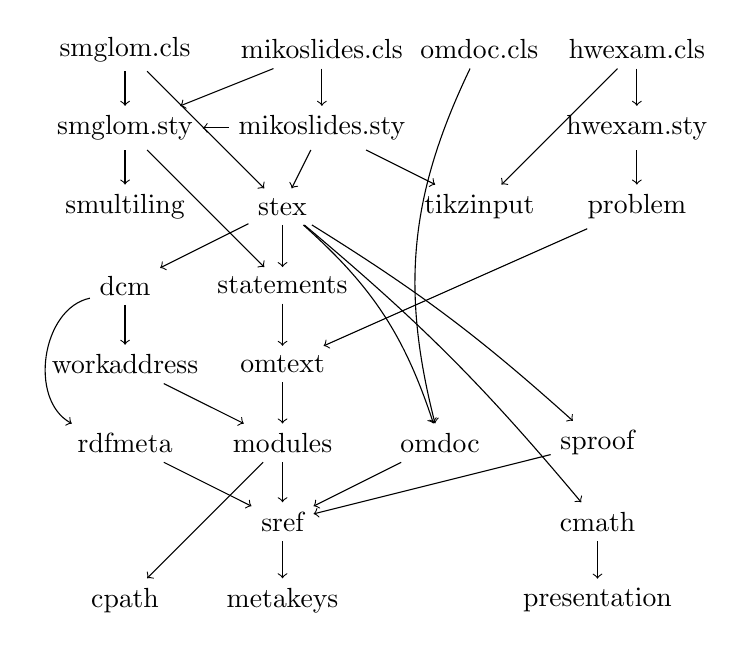
\begin{tikzpicture}
  \node (metakeys) at (0,0) {metakeys};
  \node (cpath) at (-2,0) {cpath};
  \node (presentation) at (4,0) {presentation};

  \node (sref) at (0,1) {sref};
  \node (cmath) at (4,1) {cmath};

  \node (rdfmeta) at (-2,2) {rdfmeta};
  \node (modules) at (0,2) {modules};
  \node (omdoc) at (2,2)  {omdoc};
  \node (sproof) at (4,2)  {sproof};

  \node (wa) at (-2,3) {workaddress};
  \node (omtext) at (0,3) {omtext};

  \node (dcm) at (-2,4) {dcm};
  \node (statements) at (0,4) {statements};
  \node (problem) at (4.5,5) {problem};
  \node (tikzinput) at (2.5,5) {tikzinput};

  \node (stex) at (0,5) {stex};
  \node (smultiling) at (-2,5) {smultiling};

  \node (smglomsty) at (-2,6) {smglom.sty};
  \node (mikoslidessty) at (.5,6) {mikoslides.sty};
  \node (hwexamsty) at (4.5,6) {hwexam.sty};

  \node (smglomcls) at (-2,7) {smglom.cls};
  \node (mikoslidescls) at (.5,7) {mikoslides.cls};
  \node (hwexamcls) at (4.5,7) {hwexam.cls};
  \node (omdoccls) at (2.5,7) {omdoc.cls};

  \draw[->] (sref) -- (metakeys);
  \draw[->] (cmath) -- (presentation);
  \draw[->] (rdfmeta) -- (sref);
  \draw[->] (wa) -- (modules);
  \draw[->] (modules) -- (sref);
  \draw[->] (modules) -- (cpath);
  \draw[->] (omdoc) -- (sref);
  \draw[->] (sproof) -- (sref);
  \draw[->] (dcm) to[bend right=70] (rdfmeta);
  \draw[->] (dcm) -- (wa);
  \draw[->] (omtext) -- (modules);
  \draw[->] (statements) -- (omtext);
  \draw[->] (stex) -- (statements);
  \draw[->] (stex) -- (dcm);
  \draw[->] (stex) to[bend left=5] (sproof);
  \draw[->] (stex) to[bend left=5] (cmath);
  \draw[->] (stex) to[bend left=15] (omdoc);
  \draw[->] (problem) -- (omtext);
  \draw[->] (smglomsty) -- (smultiling);
  \draw[->] (smglomsty) -- (statements);
  \draw[->] (smglomcls) -- (smglomsty);
  \draw[->] (smglomcls) -- (stex);
  \draw[->] (mikoslidescls) -- (mikoslidessty);
  \draw[->] (mikoslidescls) -- (smglomsty);
  \draw[->] (mikoslidessty) -- (tikzinput);
  \draw[->] (mikoslidessty) -- (stex);
  \draw[->] (mikoslidessty) -- (smglomsty);
  \draw[->] (hwexamcls) -- (hwexamsty);
  \draw[->] (hwexamsty) -- (problem);
  \draw[->] (omdoccls) to[bend right=20] (omdoc);

  \draw[->] (hwexamcls) -- (tikzinput);
\end{tikzpicture}
\caption{The \sTeX packages and their dependencies.}
\end{figure}
\subsection{Mathematical Statements}

\subsubsection{{\texttt{statements}}: Extending Content Macros for Mathematical Notation}
 
The \texttt{statements} package (see\ctancite{Kohlhase:smms}) provides semantic markup
facilities for mathematical statements like Theorems, Lemmata, Axioms, Definitions,
etc. in {\stex} files. This structure can be used by MKM systems for added-value services,
either directly from the {\sTeX} sources, or after translation.

\subsubsection{{\texttt{sproof}}: Extending Content Macros for Mathematical Notation}
 
The \texttt{sproof} package (see~\ctancite{Kohlhase:smp})supplies macros and environment
that allow to annotate the structure of mathematical proofs in {\stex} files. This
structure can be used by MKM systems for added-value services, either directly from the
{\sTeX} sources, or after translation.


\subsection{Context Markup for Mathematics}

\subsubsection{{\texttt{modules}}: Extending Content Macros for Mathematical Notation}
 
The \texttt{modules} package (see~\ctancite{KohAmb:smmssl}) supplies a definition
mechanism for semantic macros and a non-standard scoping construct for them, which is
oriented at the semantic dependency relation rather than the document structure. This
structure can be used by MKM systems for added-value services, either directly from the
{\sTeX} sources, or after translation.

\subsection{Mathematical Document Classes}

\subsubsection{Connexions Modules}

{\cnxlatex} (see~\ctancite{Kohlhase:clbscm}) is a collection of {\LaTeX} macros that allow
to write {\connexions} modules without leaving the {\LaTeX} workflow. Modules are authored
in {\cnxlatex} using only a text editor, transformed to PDF and proofread as usual. In
particular, the {\LaTeX} workflow is independent of having access to the {\connexions}
system, which makes {\cnxlatex} attractive for the initial version of single-author
modules.


For publication, {\cnxlatex} modules are transformed to {\cnxml} via the {\latexml}
translator and can be uploaded to the {\connexions} system.

\subsubsection{OMDoc Documents}

The \texttt{omdoc} package provides an infrastructure that allows to markup {\omdoc}
documents in {\LaTeX}. It provides \texttt{omdoc.cls}, a class with the and
{\texttt{omdocdoc.sty}}

\subsection{Conclusion}\label{sec:concl}

The {\stex} collection provides a set of semantic macros that extends the familiar and
time-tried {\LaTeX} workflow in academics until the last step of Internet publication of
the material. For instance, a {\connexions} module can be authored and maintained in
{\LaTeX} using a simple text editor, a process most academics in technical subjects are
well familiar with. Only in a last publishing step (which is fully automatic) does it get
transformed into the {\xml} world, which is unfamiliar to most academics. 

Thus, {\stex} can serve as a conceptual interface between the document author and MKM
systems: Technically, the semantically preloaded {\LaTeX} documents are transformed into
the (usually {\xml}-based) MKM representation formats, but conceptually, the ability to
semantically annotate the source document is sufficient.
 
The {\stex} macro packages have been validated together with a case
study~\cite{Kohlhase04:stex}, where we semantically preload the course materials for a
two-semester course in Computer Science at Jacobs University Bremen and transform them to
the {\omdoc} MKM format.

\subsection{Licensing, Download and Setup}\label{sec:setup}
 
The {\stex} packages are licensed under the {\LaTeX} Project Public License~\cite{LPPL},
which basically means that they can be downloaded, used, copied, and even modified by
anyone under a set of simple conditions (e.g. if you modify you have to distribute under a
different name). 

The {\stex} packages and classes are available from the Comprehensive {\TeX} Archive
Network (CTAN~\cite{CTAN:on}) and are part of the primary {\TeX/\LaTeX} distributions
(e.g. TeXlive~\cite{TeXLive:on} and MikTeX~\cite{MiKTeX:on}). The development version is
on GitHub~\cite{sTeX:github:on}, it can cloned or forked from the repository URL
\begin{center}
  \url{https://github.com/KWARC/sTeX.git}
\end{center}
It is usually a good idea to enlarge the internal memory allocation of the \TeX/\LaTeX executables. This can be done by
adding the following configurations in \texttt{texmf.cnf} (or changing them, if they
alreday exist). Note that you will probably need \texttt{sudo} to do this. 
\begin{lstlisting}
max_in_open = 50        % simultaneous input files and error insertions, 
param_size = 20000      % simultaneous macro parameters, also applies to MP
nest_size = 1000        % simultaneous semantic levels (e.g., groups)
stack_size = 10000      % simultaneous input sources
main_memory = 12000000
\end{lstlisting}
After that, you have to run the 
\begin{lstlisting}
sudo fmtutil-sys --all
\end{lstlisting}

\section{Utilities}\label{sec:utilities}

To simplify dealing with {\stex} documents, we are providing a small collection of command
line utilities, which we will describe here. For details and downloads go to
{\url{http://kwarc.info/projects/stex}}.

\begin{description}
\item[{\texttt{msplit}}] splits an {\stex} file into smaller ones (one module per file)
\item[{\texttt{rf}}] computes the ``reuse factor'', i.e. how often {\stex} modules are reused
  over a collection of documents 
\item[{\texttt{sgraph}}] visualizes the module graph
\item[{\texttt{sms}}] computes the {\stex} module signatures for a give {\stex} file
\item[{\texttt{bms}}] proposes a sensible module structure for an un-annotated {\stex} file
\end{description}
\printbibliography
\end{document}
%%% Local Variables: 
%%% mode: LaTeX
%%% TeX-master: t
%%% End: 

% LocalWords:  hoc LaTeXML nC CSumLimits cmathml DVI th sproof dtx mikoslides 2oms04 ci
% LocalWords:  ltxml pdf texhash mktexlsr MikTEX msplit rf sgraph sms bms un eq RobVor ci
% LocalWords:  cnx omdoc pagenumbering maketitle setcounter tocdepth clearpage Lamport
% LocalWords:  tableofcontents openmath omfmd05 Bergstra mathml ttb84 ladps94 StaGinDav
% LocalWords:  xslt Deach exls99 xpr00 stex ednote mathcal twintoo CSumlLimits maacl09
% LocalWords:  infty Cexp qquad hbox qquad exfig lstlisting belowskip aboveskip sumlimits
% LocalWords:  xmlns bvar bvar lowlimit cn cn lowlimit uplimit uplimit exp tt inparaenum
% LocalWords:  subsubsection texttt ctancite tbscml ipsmsl smms smp KohAmb searchabiliby
% LocalWords:  smmssl cnxlatex clbscm cnxml omdoc.cls omdocdoc.sty concl TeXlive TeXLive
% LocalWords:  printbibliography
